\subsection{Granularity of Variability}
\begin{frame}{\myframetitle}
	\begin{mycolumns}[animation=none]
		\mydefinition{Granularity of Variability}{
			\begin{itemize}
				\item Depending on the implementation technique, variability can be introduced at different levels of granularity.
				\item A level of granularity refers to
				\begin{itemize}
					\item the hierarchical organization of implementation artifacts (e.g., through the file system),
					\item the hierarchical structure of an implementation artifact (e.g., given by its syntax)
				\end{itemize}
			\end{itemize}
		}
		\myexample{Granularity Levels in Java}{
			Archives $>$ packages $>$ classes $>$ members $>$ statements
		}
		\pause
	\mynextcolumn
		\mynote{What we have seen so far?}{
			\begin{itemize}
				\item Coarse-grained: Clone-and-own with version control (entire variants)
				\item Medium-grained: Clone-and-own with build systems (file level)
				\item Medium-grained: Features with build systems (file level)
				\item Medium-grained: Design patterns for variability (class or member level)
				\item Fine-grained: Runtime parameters (statement level) 
			\end{itemize}
		}
		\pause
		\mynote{What is missing?}{
			Yet no approach supporting fine-grained compile-time variability!
		}		
	\end{mycolumns}
\end{frame}
% Christian's paper?
% empirical studies?
% essence: file-level variability is not engough

\subsection{What is a Preprocessor?}
\begin{frame}{\myframetitle\mysource{\fospl\mypages{110--111}}}
	\begin{mycolumns}
		\begin{definition}{Preprocessor}
			\begin{itemize}
				\item tool manipulating source code before compilation (i.e., at compile time)
				\item preprocessors are used:
					\begin{itemize}
						\item to inline files\hfill(e.g., header files)
						\item to define and expand macros\\\hfill(cf.\ metaprogramming)
						\item for \textbf{conditional compilation}\\\hfill(e.g., remove debug code for release)
					\end{itemize}
			\end{itemize}
		\end{definition}
	\mynextcolumn
		\begin{note}{Preprocessor}
			\begin{itemize}
				\item the C Preprocessor is used in almost every C/C++ project
				\item preprocessors are typically oblivious to the target language as they operate on text files (e.g., the C Preprocessor can also used for Fortran or Java)
				\item conditional compilation is a very common technique to implement product lines
			\end{itemize}
		\end{note}
	\end{mycolumns}
\end{frame}

% in-place vs outa-place preprocessors
% how to select features? parameters passed to the preprocessor, define in source code

\subsection{CPP -- The C Preprocessor}
\begin{frame}{\myframetitle\ -- In a Nutshell \mytitlesource{\featureide}}
	\leftorright{
		\myexampletight{Example Input to the Preprocessor}{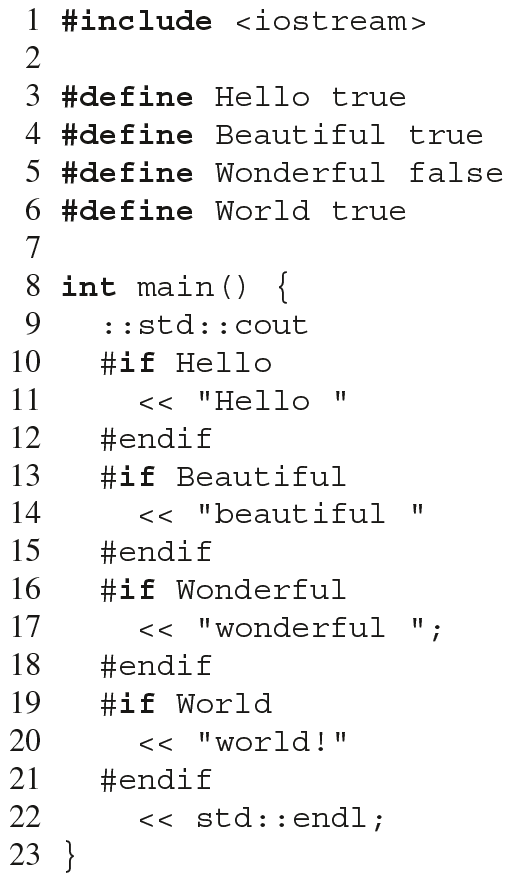
\includegraphics[scale=.3]{preprocessor-c}}
	}{
		\myexampletight{Example Output (Simplified)}{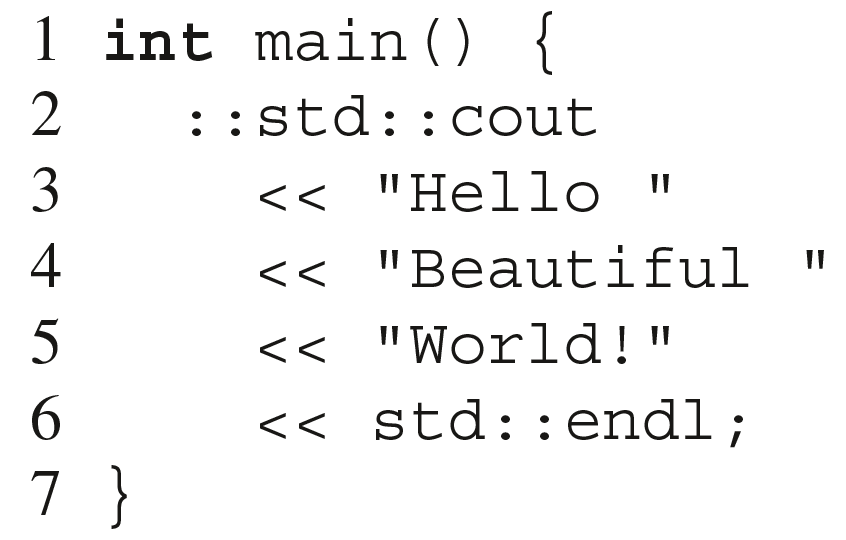
\includegraphics[scale=.15]{preprocessor-c-output}}
		\begin{note}{}
			preprocessors typically do not remove line breaks to not influence of line numbers reported by compilers
		\end{note}
	}
\end{frame}
% TODO example contains "Beautiful" but should be "beautiful"
% TODO keywords: #ifdef #endif #else
% TODO illustrate parameters and the call of the preprocessor

\begin{frame}{\myframetitle\ -- In a Coconutshell}
	\todots
\end{frame}
% TODO explain the most important commands: #if #defined or and not ... #elif
% TODO #include

% TODO #error
% TODO parameters, #define, even combinations

% TODO single characters
% TODO discipliced, undisciplined

\subsection{Preprocessors for Java}
\begin{frame}{Munge -- A Simple Preprocessor for Java \mytitlesource{\featureide}}
	\begin{mycolumns}[widths={55}]
		\myexampletight{Example Input and Output}{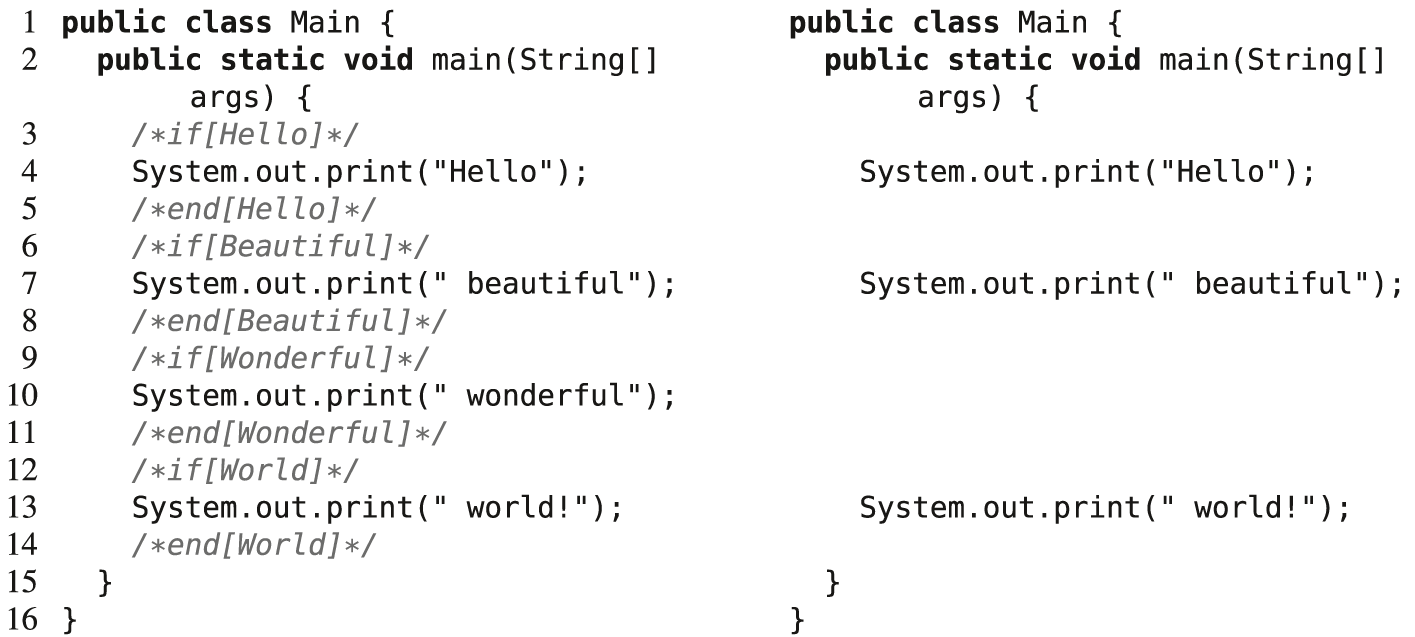
\includegraphics[width=\linewidth]{preprocessor-munge}}
	\mynextcolumn
		\myexampletight{Calling the Preprocessor}{
			\centering
			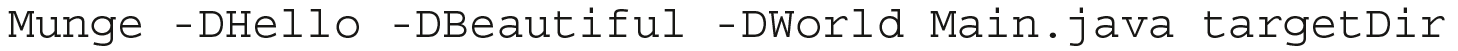
\includegraphics[width=\linewidth]{preprocessor-munge-call}
			
			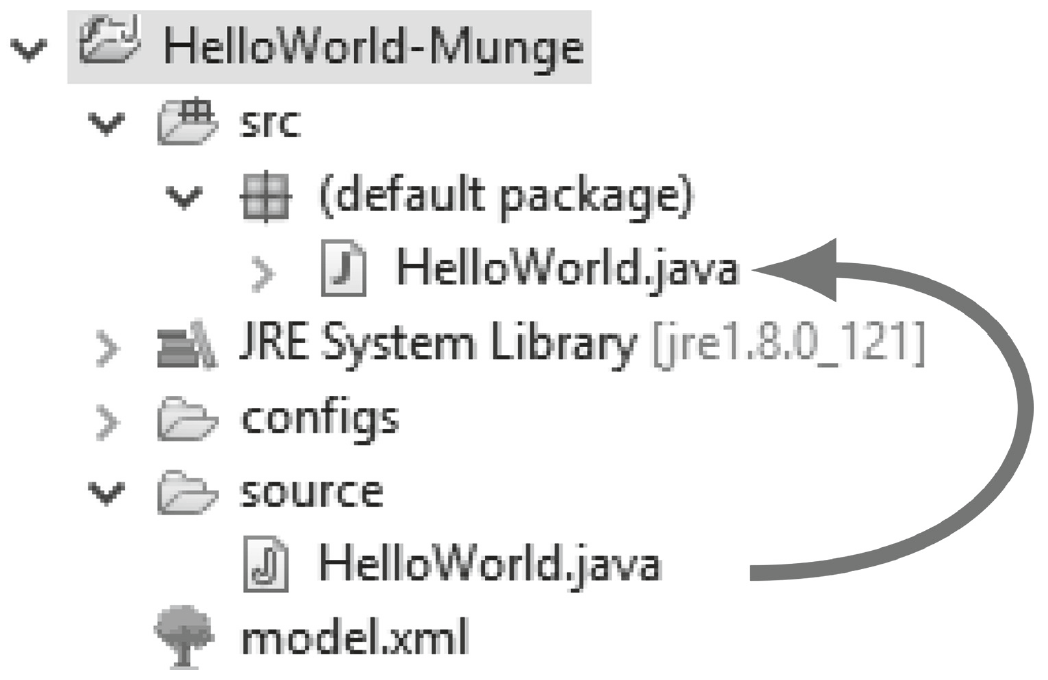
\includegraphics[width=.7\linewidth]{preprocessor-munge-idea}
		}
	\end{mycolumns}
\end{frame}

\begin{frame}{Antenna -- An In-Place Preprocessor for Java \mytitlesource{\featureide}}
	\begin{mycolumns}[widths={55}]
		\myexampletight{Example Input and Output}{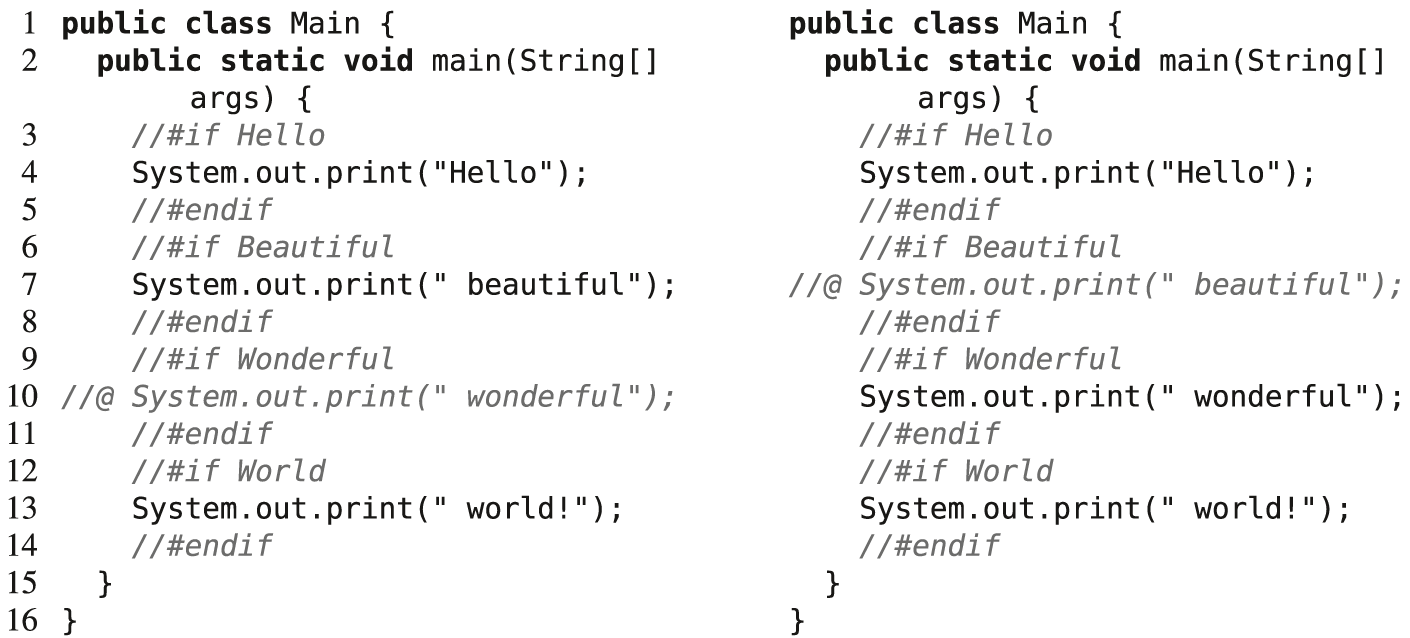
\includegraphics[width=\linewidth]{preprocessor-antenna}}
	\mynextcolumn
		\myexampletight{Calling the Preprocessor}{
			\centering
			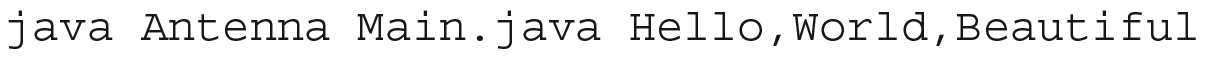
\includegraphics[width=\linewidth]{preprocessor-antenna-call}
			
			~
			
			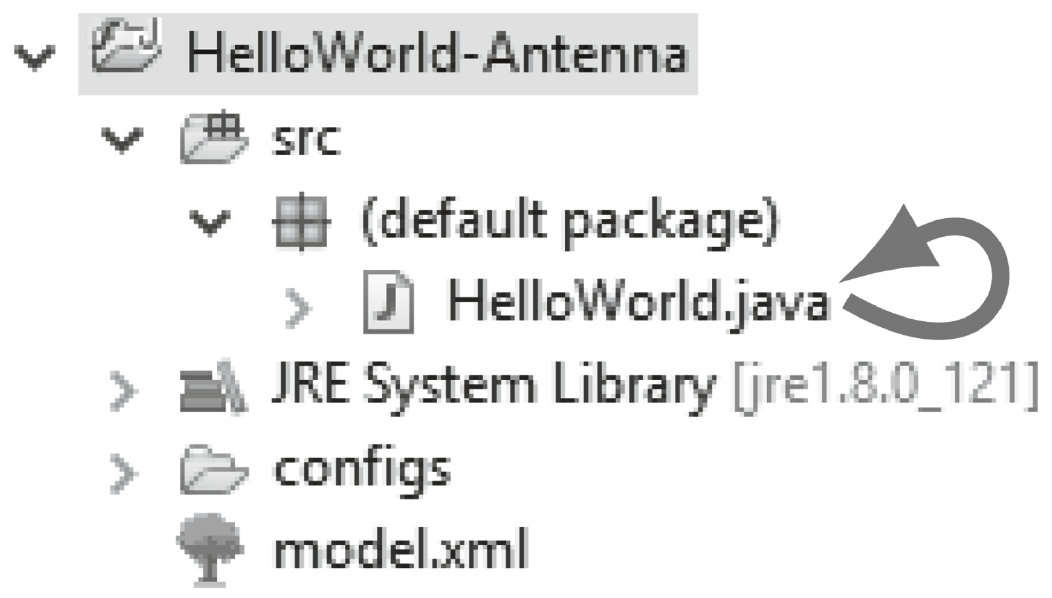
\includegraphics[width=.7\linewidth]{preprocessor-antenna-idea}
		}
	\end{mycolumns}
\end{frame}

\subsection{Preprocessors in FeatureIDE}
\begin{frame}{\myframetitle\mysource{\featureide}}
	\begin{mycolumns}[animation=none,widths={75}]
		\only<1|handout:0>{\pic[width=\linewidth]{featureide-antenna-featuremodel}}%
		\only<2|handout:1>{\pic[width=\linewidth]{featureide-antenna-configuration}}%
		\only<3|handout:0>{\pic[width=\linewidth]{featureide-antenna-warning}}%
		\only<4|handout:0>{\pic[width=\linewidth]{featureide-antenna-contentassist}}%
	\mynextcolumn
%		\begin{definition}{FeatureIDE\mysource{\featureide}}
%			\begin{itemize}
%				\item 
%			\end{itemize}
%		\end{definition}
		\begin{note}{\href{https://www.youtube.com/watch?v=jVe7f32mLCQ}{Demo Video}}
			\begin{itemize}
				\item preprocessing with Antenna on command line
				\item feature modeling
				\item warnings for unreferenced features
				\item content assist proposing feature names
				\item configuration and automated regeneration
				\item (first 2 min relevant here)
			\end{itemize}
		\end{note}
	\end{mycolumns}
\end{frame}
% TODO has FeatureIDE been shown/discussed before? ideally, here only present preprocessor integration

\subsection{Discussion of Preprocessors}
\begin{frame}{\myframetitle\ \mytitlesource{\featureide}}
	\leftorright{
		\myexampletight{A Slightly More Complex Example}{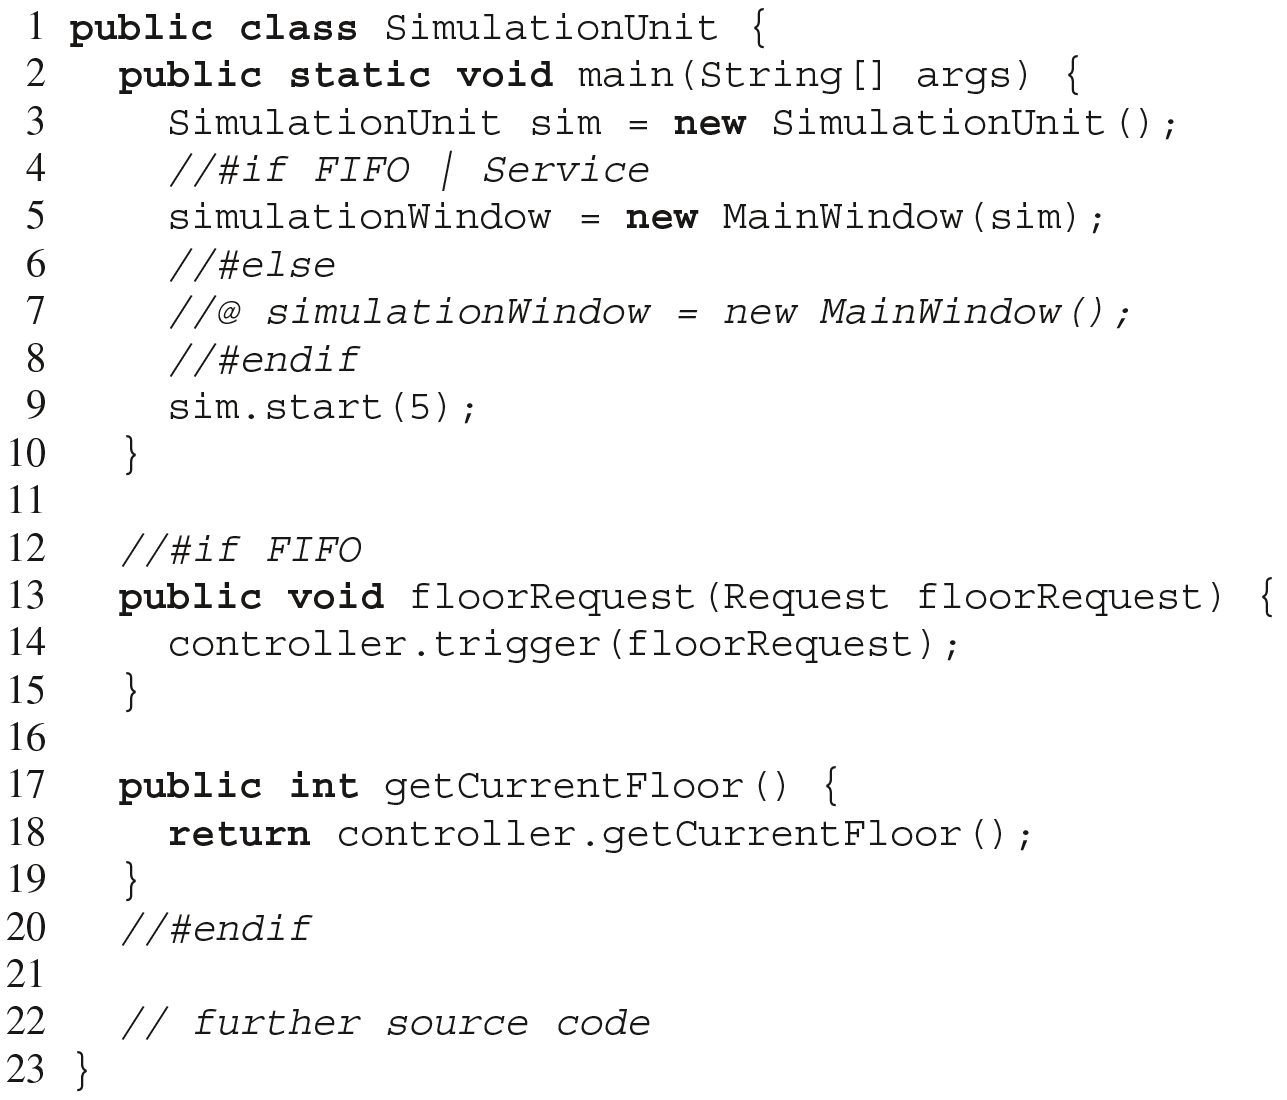
\includegraphics[width=\linewidth]{preprocessor-antenna-elevator}}
	}{
		\todots
	}
\end{frame}
% pros: fine granular, language-independent
% cons: IDE support, easy to create mistakes

\begin{frame}{Problem: Source-Code "`Obfuscation"'}
	\begin{mycolumns}[animation=none]
		\mynote{Observations on readability}{
			\begin{itemize}
				\item Mixing two languages (C and \#ifdefs, or Java and Munge, ...)
				\item Control flow difficult to understand
				\item Long annotations hard to find
				\item Extra line breaks destroy layout
			\end{itemize}
		}
	\mynextcolumn
		\todots		
	\end{mycolumns}
\end{frame}

\begin{frame}{Discussion of Features with Preprocessors}
	\begin{mycolumns}[animation=none]
		\mynote{Advantages}{
			\begin{itemize}
				\item Well-known and mature tools, readily available
				\item Easy to use; annotate and remove
				\item Support compile-time variability
				\item Flexible, arbitrary levels of granularity
				\item Can handle code and non-code artifacts
				\item Little preplanning required; variability can be added to an existing project				
			\end{itemize}
		}
	\mynextcolumn
		\pause
		\mynote{Challenges}{
			\begin{itemize}
				\item Scattering and tangling; no separation of cencerns
				\item Multiple languages intermixed in the same development artifact;
				\item May obfuscate source code and severly impact its readability
				\item Hard to analyze and process for existing IDEs
				\item Often used in an ad-hoc or undisciplined fashion
				\item Prone to subtle errors which are hard to detect				
			\end{itemize}
		}
	\end{mycolumns}
\end{frame}

\xkcdframe{619} % linux features 20s

\subsection{Preprocessor-Based Product Lines in the Wild}
\begin{frame}{\myframetitle\mysource{\fortyproductlines}}
	\leftorright{
		\begin{exampletight}{Number of Features}
			\centering\pic[width=.8\linewidth,page=1]{fortyproductlines}\\Lines of Code
		\end{exampletight}
	}{
		\begin{exampletight}{Percentage of Variable Code}
			\centering\pic[width=.8\linewidth,page=2]{fortyproductlines}\\Lines of Code
		\end{exampletight}
	}
\end{frame}

\begin{frame}{\myframetitle\mysource{\fortyproductlines}}
	\leftorright{
		\begin{exampletight}{Lines of Variable Code}
			\centering\pic[width=.8\linewidth,page=3]{fortyproductlines}\\Number of Features
		\end{exampletight}
	}{
		\begin{exampletight}{Average Nesting Depth}
			\centering\pic[width=.8\linewidth,page=6]{fortyproductlines}\\Number of Features
		\end{exampletight}
	}
\end{frame}

\begin{frame}{\myframetitle\mysource{\fortyproductlines}}
	\leftorright{
		\begin{exampletight}{Average Number of Feature References}
			\centering\pic[width=.8\linewidth,page=4]{fortyproductlines}\\Number of Features
		\end{exampletight}
	}{
		\begin{exampletight}{Average Number of Features per Annotation}
			\centering\pic[width=.8\linewidth,page=5]{fortyproductlines}\\Number of Features
		\end{exampletight}
	}
\end{frame}
% TODO create own plots for the data?
% TODO add pictures from Rodrigues et al. @ INFSOF’16 (Assessing fine-grained feature dependencies): methods with directives vs product lines

